\documentclass[11pt,a4paper]{article}
\usepackage[T1]{fontenc}
\usepackage[utf8]{inputenc}
\usepackage{lmodern}
\usepackage{amsmath,amssymb,amsthm,mathtools,mathrsfs}
\usepackage{graphicx,float,xcolor,multicol}
\usepackage[shortlabels]{enumitem}
\usepackage[margin=27mm]{geometry}
\usepackage{microtype,needspace,placeins}
\usepackage{tikz,tikz-cd}
\usetikzlibrary{arrows.meta,calc,positioning,patterns,decorations.pathreplacing}
\usepackage[colorlinks=true,linkcolor=teal,urlcolor=teal,citecolor=teal]{hyperref}
\setlength{\parindent}{0pt}
\setlength{\parskip}{.6em}
\setcounter{secnumdepth}{0}
\allowdisplaybreaks
\raggedbottom
\providecommand{\cross}{\times}
\DeclareUnicodeCharacter{2020}{\ensuremath{\dagger}}
\DeclareMathOperator{\supp}{supp}
\DeclareMathOperator*{\esssup}{ess\,sup}
\providecommand{\chapter}{\section}
\newenvironment{tool}[2]{\subsection*{Tool #1 --- #2}}{}
\newcommand{\ToolRef}[1]{Tool #1}
\newcommand{\FigureTag}[2]{\textit{Figure #1}}
\newcommand{\Result}[1]{\subsection*{#1}}
\newcommand{\Application}[1]{\subsubsection*{Application\if\relax\detokenize{#1}\relax\else\space--- #1\fi}}
\newcommand{\ProofHeading}{\par\textit{Proof.}\space}
\newcommand{\ProofOf}[1]{\par\textit{Proof of #1.}\space}
\newcommand{\RemarkHeading}{\par\textbf{Remark.}\space}
\newcommand{\NoteHeading}{\par\textbf{Note.}\space}
\newcommand{\ExerciseHeading}{\par\textbf{Exercise.}\space}

% Rendering support only; mathematical text is in each independent post.
\usepackage{booktabs,array,longtable}
\definecolor{HandoutBlue}{HTML}{2F6690}
\definecolor{HandoutNavy}{HTML}{17365D}
\newtheorem{theorem}{Theorem}
\newtheorem{lemma}[theorem]{Lemma}
\newtheorem{proposition}[theorem]{Proposition}
\newtheorem{corollary}[theorem]{Corollary}
\newtheorem{conjecture}[theorem]{Conjecture}
\newtheorem{definition}{Definition}
\newtheorem{example}{Example}
\newtheorem{namedtoolcounter}{Tool}
\newenvironment{namedtool}[1]{\begin{namedtoolcounter}[#1]}{\end{namedtoolcounter}}
\newtheorem*{claim}{Claim}
\newtheorem*{remark}{Remark}
\newtheorem*{exercise}{Exercise}
\newtheorem*{question}{Question}
\newtheorem*{observation}{Observation}
\newcommand{\SourceChapter}[2]{\section*{#2}}
\newcommand{\Lecture}[2]{\section*{Lecture #1: #2}}
\newcommand{\unclear}[1]{\textit{[unclear: #1]}}
\newcommand{\sourcegap}{\textit{[unfinished in the source]}}
\DeclareMathOperator{\dist}{dist}
\DeclareMathOperator{\id}{id}
\DeclareMathOperator{\Hol}{Hol}
\DeclareMathOperator{\Per}{Per}
\DeclareMathOperator{\Fix}{Fix}
\DeclareMathOperator{\diam}{diam}
\DeclareMathOperator{\Var}{Var}
\DeclareMathOperator{\Leb}{Leb}
\DeclareMathOperator{\Hom}{Hom}
\DeclareMathOperator{\End}{End}
\DeclareMathOperator{\Ann}{Ann}
\DeclareMathOperator{\Spec}{Spec}
\DeclareMathOperator{\Max}{Max}
\DeclareMathOperator{\Ob}{Ob}
\DeclareMathOperator{\Tor}{Tor}
\DeclareMathOperator{\Ass}{Ass}
\DeclareMathOperator{\Mor}{Mor}
\DeclareMathOperator{\Fun}{Fun}
\DeclareMathOperator{\Nat}{Nat}
\DeclareMathOperator{\Cone}{Cone}
\DeclareMathOperator{\MCG}{MCG}
\DeclareMathOperator{\Aut}{Aut}
\DeclareMathOperator{\Deck}{Deck}
\DeclareMathOperator{\SL}{SL}
\DeclareMathOperator{\PSL}{PSL}
\DeclareMathOperator{\Area}{Area}
\DeclareMathOperator{\im}{im}
\DeclareMathOperator{\PSh}{PSh}
\newcommand{\CRing}{\mathsf{CRings}}
\newcommand{\AMod}{A\text{-}\mathsf{Mod}}
\newcommand{\Ab}{\mathsf{Ab}}
\newcommand{\Z}{\mathbb Z}
\newcommand{\Q}{\mathbb Q}
\newcommand{\R}{\mathbb R}
\newcommand{\C}{\mathbb C}
\newcommand{\N}{\mathbb N}
\newcommand{\kk}{\mathbb k}
\renewcommand{\aa}{\mathfrak a}
\newcommand{\bb}{\mathfrak b}
\newcommand{\pp}{\mathfrak p}
\newcommand{\qq}{\mathfrak q}
\newcommand{\mm}{\mathfrak m}
\newcommand{\nn}{\mathfrak n}
\newcommand{\rad}{\mathrm r}
\newcommand{\cat}[1]{\mathsf{#1}}
\setcounter{secnumdepth}{0}
\allowdisplaybreaks

\graphicspath{{figures/miscellaneous/}}
\begin{document}
\section*{Erdős Distance Problem}
% BLOG-CONTENT-BEGIN
% Source page 1
According to Paul Erd\H{o}s, his most important contribution to geometry is
his distance conjecture. The formulation of the problem is quite innocuous
and recreational in nature. Let me begin by stating the problem explicitly.

Let $P$ be a set of $n$ points in $\mathbb R^2$, and let
$\Delta(P):=\{|p-p'|:p,p'\in P,\ p\ne p'\}$. Thus $\Delta(P)$ is essentially
the set of possible distinct distances between distinct points.
For instance, if $P$ is the set described pictorially below, then
$\Delta(P)=\{10,2\}$.
\begin{figure}[H]
 \centering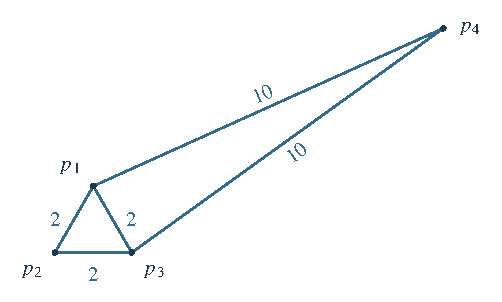
\includegraphics[width=.62\textwidth]{m2-fig-01.pdf}
 \FigureTag{M2.1}{fig:m2-fig-01}
\end{figure}
But wait! What about $|p_2-p_4|$? Is there a way to salvage this blunder?
Is there a configuration of four points such that three of them form an
equilateral triangle and the fourth one is at a distance $10$?
If you think about it for a minute, it is immediate that such a
configuration is impossible, for the fourth point $p_4$ must be the
% Source page 2
centroid of $\triangle p_1p_2p_3$, so $|p_4-p_i|<2$ for every $1\le i\le3$.
If you think about it a bit more, you will realise that all configurations
of four points in $\mathbb R^2$ must have at least two distinct distances.
Why? Set $P=\{p_1,p_2,p_3,p_4\}$.

Given four points $p_1,p_2,p_3,p_4$, we have $\binom42=6$ nonzero distances.
If $|\Delta(P)|=1$, any three of the points form an equilateral triangle;
the fourth point would have to be a second point at the same distance from
all three vertices, which is impossible in the plane.
This argument just showed us that the plane is rigid: it does not allow
points on it to float around with an arbitrary set of distinct distances.

As interesting as it may be to ask which sets of distances can be realised
in $\mathbb R^2$, let us begin by asking the following.
\begin{question}
What is $\inf_{|P|=n}|\Delta(P)|$? If $g(n):=\inf_{|P|=n}|\Delta(P)|$ is
the minimum number of possible distances, describe $g(n)$.
\end{question}
We know $g(0)=0$, $g(1)=0$, $g(2)=1$, $g(3)=1$ (an equilateral triangle),
$g(4)=2$, $g(5)=2$ (a pentagon), and so on.
Erd\H{o}s was particularly interested in trying to find bounds for $g(n)$,
both upper and lower bounds; he was not optimistic enough to look for
asymptotes.

% Source page 3
He believed that $g(n)$ must roughly behave like $n$ for large $n$.
It is firstly easy to see that, mostly, $|\Delta(P)|$ will be like $|P|^2$,
because we can consider the following function (let $|P|=n$):
\[
 F\colon\underbrace{\mathbb R^2\times\mathbb R^2\times\cdots\times\mathbb R^2}_{n\text{ times}}
 \longrightarrow\mathbb R,
\]
\[
 F(p_1,\ldots,p_n):=
 \prod_{\substack{1\le i<j\le n,\ 1\le k<\ell\le n\\(i,j)<(k,\ell)}}
 \bigl(|p_i-p_j|^2-|p_k-p_\ell|^2\bigr).
\]
$F$ is nonzero on a dense open set in $\mathbb R^{2n}$. On that dense open
set, the points $p_1,p_2,\ldots,p_n$ are distinct and all their pairwise
distances are distinct. Thus $|\Delta(P)|=\binom n2$ there.
Forget those, because we are interested in $g(n)$. The reason Erd\H{o}s
believed that $g(n)$ is roughly linear is that he was able to come up with
a configuration of $n$ points, for every $n$, such that $|\Delta(P)|\sim n$.
Indeed, if $P=\{(0,1),(1,1),\ldots,(n-1,1)\}$, then $|\Delta(P)|=n-1$.
Thus $g(n)\le n-1$ trivially, but Erd\H{o}s was able to beat this by
considering the following clever arrangement.
For $N=m^2$, he considered the integer grid
$P=\{0,1,\ldots,m-1\}^2$, as shown below.
\begin{figure}[H]
 \centering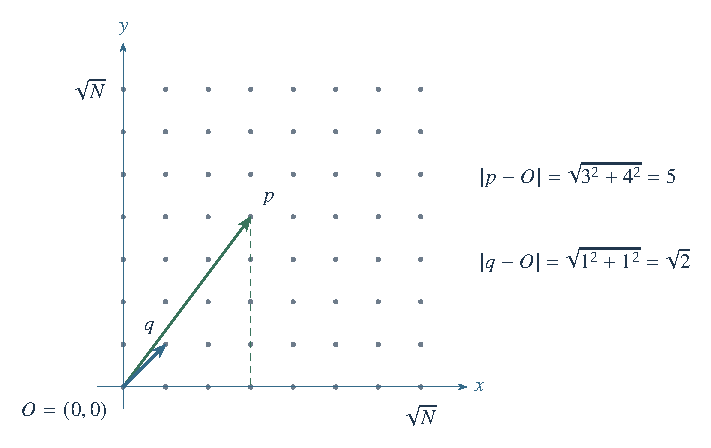
\includegraphics[width=.72\textwidth]{m2-fig-02.pdf}
 \FigureTag{M2.2}{fig:m2-fig-02}
\end{figure}

% Source page 4
We have
\[
 \Delta(P)=\{\sqrt A:A=x^2+y^2,\ 0\le x,y\le m-1,\ A>0\}
 \quad\Longrightarrow\quad 1\le A<2N.
\]
Notice that $|\Delta(P)|$ is at most the number of positive integers below
$2N$ that are sums of two squares.
Therefore
\[
 g(N)\le\bigl|\{1\le k<2N:k\text{ is a sum of two squares}\}\bigr|.
\]
The expression on the right is usually denoted by $\pi_2(2N)$. Let us give
a rough heuristic for $\pi_2(2N)$ using very elementary number theory.
\begin{theorem}[Two Squares Theorem]
$n$ is a sum of two squares if and only if, for every prime $p\mid n$
such that $p\equiv3\pmod4$, we have $2\mid\nu_p(n)$.
\end{theorem}
We shall not digress and give a proof, for it can be found in many standard
texts in number theory. Instead, we shall use the theorem to roughly
sketch an estimate for $\pi_2(M)$.

From the integers up to $M$, we must remove all odd powers of $p$ and their
multiples, where $p\equiv-1\pmod4$. Note that this is equivalent to combining
all the even powers of $p$ and their multiples, where
$p\equiv-1\pmod4$. Let us do that via inclusion--exclusion!
Given a prime $p\le M$, the quantity $M(1-1/p)$ is roughly the number of
integers at most $M$ not divisible by $p$. Similarly, the proportion for
which the exponent of $p$ is even is
\[
 \left(1-\frac1p\right)
 \left(1+\frac1{p^2}+\frac1{p^4}+\cdots\right)
 =1-\frac1p+\frac1{p^2}-\frac1{p^3}+\cdots
 =\frac p{p+1}.
\]
% Source page 5
The notebook first extends the inclusion--exclusion principle and writes
\[
 M-\frac Mp+\frac M{p^2}-\frac M{p^3}+\frac M{p^4}-\frac M{p^5}+\cdots
 \approx M\left(1-\frac1p\right)\left(1+\frac1{p^2}\right)
 \left(1-\frac1{p^3}\right)\left(1+\frac1{p^4}\right)\cdots.
\]
The correction sum will be something of the form
$\sum_{2\nmid k}P(k)/p^k$, where $P(k)$ is the partition function.
But let us ignore that, says the notebook, for $P(k)<k^2$ and
$\sum_k k^2/p^k$ converges. This is only a heuristic: the displayed infinite
product is not an identity, and $P(k)<k^2$ does not hold for all $k$.

The exact local density used to clarify that heuristic is $p/(p+1)$, as
computed above. Extending it over the primes $p\equiv-1\pmod4$ and ignoring
the error terms from the integer parts, one obtains
\[
 \pi_2(M)\approx
 M\prod_{\substack{p\le M\\p\equiv-1\ (4)}}\frac p{p+1}.
\]
But
\[
 \frac p{p+1}=\left(1-\frac1p\right)
 \left(1+O\left(\frac1{p^2}\right)\right).
\]
The product of the second factors converges, so
\[
 \pi_2(M)\approx
 M\prod_{\substack{p\le M\\p\equiv-1\ (4)}}
 \left(1-\frac1p\right).
\]
One can now prove that
\[
 \prod_{\substack{p\le M\\p\equiv-1\ (4)}}
 \left(1-\frac1p\right)
 \approx\frac1{\sqrt{\log M}}.
\]
Again, refer to any standard text in analytic number theory for a proof.
The reason we have $1/2$ in the exponent of $\log M$ can roughly be
explained by the following, again vague, argument.
The expression $M\prod_{p\le\sqrt M}(1-1/p)$ counts the non-composite
numbers roughly and is approximately $M/\log M$. Hence, by the Prime Number Theorem,
$\prod_{p\le M}(1-1/p)\approx1/\log M$.
Now, as primes are equidistributed modulo $4$ between $1$ and $-1$,
\[
 \prod_{\substack{p\le M\\p\equiv1\ (4)}}\left(1-\frac1p\right)
 \approx
 \prod_{\substack{p\le M\\p\equiv-1\ (4)}}\left(1-\frac1p\right)
 \quad\Longrightarrow\quad
 \prod_{\substack{p\le M\\p\equiv-1\ (4)}}\left(1-\frac1p\right)
 \approx\frac1{\sqrt{\log M}}.
\]
% Source page 6
Anyway, coming back to our problem, we now roughly know that
\[
 g(N)\le \pi_2(2N)\approx\frac{2N}{\sqrt{\log(2N)}}
 \approx\frac N{\sqrt{\log N}}
 \quad\Longrightarrow\quad
 g(N)=O\left(\frac N{\sqrt{\log N}}\right).
\]
Erd\H{o}s was thus able to get this neat bound from an observation purely
number-theoretic in nature. We now have a strong reason to believe that a
lower bound roughly of order $n^{1-\varepsilon}$ must exist for every
$\varepsilon>0$. This conviction led him to conjecture the following.

\setcounter{theorem}{2}\begin{conjecture}[Erd\H{o}s Distance Conjecture]
For every $c<1$, $g(n)=\Omega(n^c)$. This means that
\[
 \text{there exist $C>0$ and $N_0$ such that }g(n)\geq Cn^c
 \text{ for every }n\geq N_0.
\]
\end{conjecture}
A colloquial way of saying it is that $g(n)$ is roughly $n$, up to a
logarithmic decay.
\begin{remark}
This slick observation of Erd\H{o}s fails when you go to, say, $\mathbb R^4$,
for, by Lagrange's Four-Square Theorem, every number is a sum of four
squares. There number theory will not give you a logarithmic decay.
\end{remark}
Getting an upper bound is easy; we just did it:
$g(n)\le cn/\sqrt{\log n}$. What proved to be extremely difficult was to
get a lower bound, because that must use the dimension of the manifold
one is dealing with very crucially: $g(4)=1$ in $\mathbb R^3$ (a tetrahedron).
% Source page 7
The arguments must crucially use the fact that the dimension is $2$ and
the manifold is $\mathbb R^2$, for even on a sphere a tetrahedron can be
arranged, forcing $g(4)=1$. We must use the fact that the points are not
only in a two-dimensional manifold: they are in $\mathbb R^2$.

The best lower bound one expects for $g(n)$ is $cn/\sqrt{\log n}$ for
some $c$ and large $n$. People do not try to prove $g(n)=\Omega(n^c)$,
for the arguments are not yet structural. What they instead do is get
better and better lower bounds. Here is Erd\H{o}s's conjecture \emph{rephrased}.
\setcounter{theorem}{3}\begin{conjecture}[Lower bound]
For some $c>0$ and large $n$, $g(n)\ge cn/\sqrt{\log n}$.
\end{conjecture}
Erd\H{o}s did quite poorly in trying to come up with lower bounds, and
perhaps he did not care enough at that point to announce prize money for
this problem. I guess one can imagine him being content with just this much.
\setcounter{theorem}{4}\begin{theorem}[Erd\H{o}s, 1946]
$g(n)\ge c\sqrt n$.
\end{theorem}
\begin{proof}
Let $P$ be a configuration such that $|P|=n$, and let $p_0\in P$.
Draw $t$ circles centred at $p_0$ such that every point in $P\setminus\{p_0\}$ belongs to
one such circle and each circle has at least one point of $P\setminus\{p_0\}$.
% Source page 8
By the pigeonhole principle, at least one circle must have at least $(n-1)/t$
points of $P$. Again by the pigeonhole principle, at least one of the
semicircles must have $(n-1)/(2t)$ points. Pick the rightmost point to see that
it will have at least $(n-1)/(2t)$ distinct distances to points of $P$ on that
semicircle. Therefore
\[
 |\Delta(P)|\ge\max\left(t,\frac {n-1}{2t}\right)
 \ge\sqrt{\frac {n-1}2}.
\]
Thus $g(n)\geq c\sqrt n$ for a positive absolute constant $c$.
\end{proof}
\begin{remark}
This argument can be generalised to $\mathbb R^d$ via induction to get
$g(n)\ge cn^{1/d}$, but the conjecture for $\mathbb R^d$ is that
$g(n)\ge cn^{2/d}$, so even there this bound is quite bad!
\end{remark}
Let us now look at a slight improvement of Erd\H{o}s's lazy result.
\setcounter{theorem}{5}\begin{theorem}[Moser, 1952]
$g(n)\ge cn^{2/3}$ for some $c>0$.
\end{theorem}
\begin{proof}
Let $P$ be a configuration such that $|P|=n$. Choose $x,y\in P$ such that
$|x-y|$ is minimal. Let $O$ be the midpoint; centred at $O$, draw annuli of
% Source page 9
thickness $|x-y|$. Call these annuli $\widetilde A_1,\widetilde A_2,\ldots,
\widetilde A_\ell$, as illustrated below.
\begin{figure}[H]
 \centering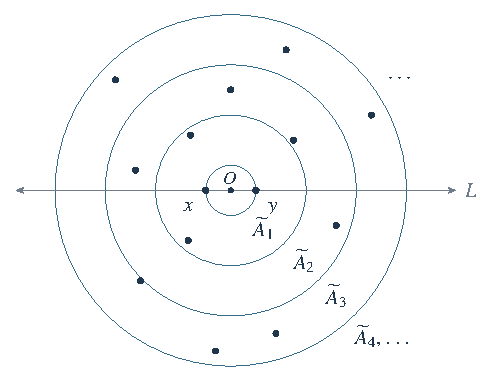
\includegraphics[width=.78\textwidth]{m2-fig-03.pdf}
 \FigureTag{M2.3}{fig:m2-fig-03}
\end{figure}
Let $L$ be the line joining $x,y$. By the pigeonhole principle, half of
$P$ is, without loss of generality, on or above the line $L$. Henceforth
$\widetilde A_i$ denotes the annuli on or above $L$.
Partition $\{\widetilde A_i\}_{i=1}^{\ell}$ into
$\{\widetilde A_i\}_{i\equiv0\ (3)}$, $\{\widetilde A_i\}_{i\equiv1\ (3)}$,
and $\{\widetilde A_i\}_{i\equiv-1\ (3)}$. By the pigeonhole principle,
one of these parts must contain at least one third of $P$, so that part
contains one sixth of $P$ above $L$.
Without loss of generality, let $\{\widetilde A_i\}_{i\equiv0\ (3)}$ be
that part. Let $\widetilde A_{3j}$ be the $j$th annulus in this part, and let
\[
 \{|p-x|:p\in\widetilde A_{3j}\}\cup
 \{|p-y|:p\in\widetilde A_{3j}\}=\{d_1,d_2,\ldots,d_k\}.
\]
If we draw circles from $x,y$ touching all points in $\widetilde A_{3j}$,
there will be $k$ of them. Let
\[
 A_i:=\{p\in\widetilde A_{3j}:|p-x|=d_i\},\qquad
 B_i:=\{p\in\widetilde A_{3j}:|p-y|=d_i\}.
\]
Then $A_i=\bigcup_{k'}(A_i\cap B_{k'})$, since every point in
$\widetilde A_{3j}$ at distance $d_i$ from $x$ is at some distance from $y$.
% Source page 10
Consequently $\bigcup_i A_i=\bigcup_{i,k'}(A_i\cap B_{k'})$.
Let $|\bigcup_{i=1}^kA_i|=n_j$. We have
\[
 \left|\bigcup_{i,k'}(A_i\cap B_{k'})\right|
 \le k^2\max_{i,k'}|A_i\cap B_{k'}|.
\]
Note that $A_i$ and $B_{k'}$ are points on circles centred at $x$ and $y$.
The two intersections are symmetric across $L$, so above $L$ we have
$|A_i\cap B_{k'}|\le1$, giving $k\ge\sqrt{n_j}$.
In the $j$th annulus $\widetilde A_{3j}$ there are therefore at least
$\sqrt{n_j}$ distinct distances from $x$ or $y$.
Notice that $\widetilde A_{3j}$ and $\widetilde A_{3j+3}$ can never have
points at the same distance from $x$ or $y$, so we can sum them together to obtain
$|\Delta(P)|\ge\sum_j\sqrt{n_j}$.
Since each $n_j$ denotes the number of points in $\widetilde A_{3j}$
above $L$, we have $n/6\le\sum_jn_j$. Thus
\[
 \frac n6\le\sum_jn_j
 \le\sum_j(\sqrt{n_j})(\sqrt{n_j})
 \le\sqrt{\max_j n_j}\sum_j\sqrt{n_j}
 \le\sqrt{\max_j n_j}\,|\Delta(P)|.
\]
The source next claims $|\Delta(P)|\ge\max_j n_j$ by choosing the rightmost
point in an annulus of maximum occupancy. The earlier rightmost-point argument,
however, applies to points on one semicircle: within an annulus the radii vary,
and two other points can be at the same distance from the chosen point. Thus the
written argument does not establish the first estimate below:
\[
 |\Delta(P)|\mathrel{\stackrel{?}{\ge}}\max_j n_j,\qquad
 |\Delta(P)|\ge\frac n{6\sqrt{\max_j n_j}}.
\]
% Source page 11
If the missing first estimate is supplied by an additional geometric argument,
then it follows that
\[
 |\Delta(P)|^2\,|\Delta(P)|
 \ge\frac{n^2}{36\max_j n_j}\max_j n_j=\frac{n^2}{36},
 \qquad
 |\Delta(P)|\ge\frac{n^{2/3}}{36^{1/3}}
 \quad\Longrightarrow\quad
 g(n)\ge\frac1{\sqrt[3]{36}}n^{2/3}.
\]
The constant here is $1/\sqrt[3]{36}$.
\end{proof}
Since Moser enhanced Erd\H{o}s's argument with quite a clever construction
of foliated annuli, many joined the race to get to the bound $cn/\sqrt{\log n}$.
\begin{figure}[H]
 \centering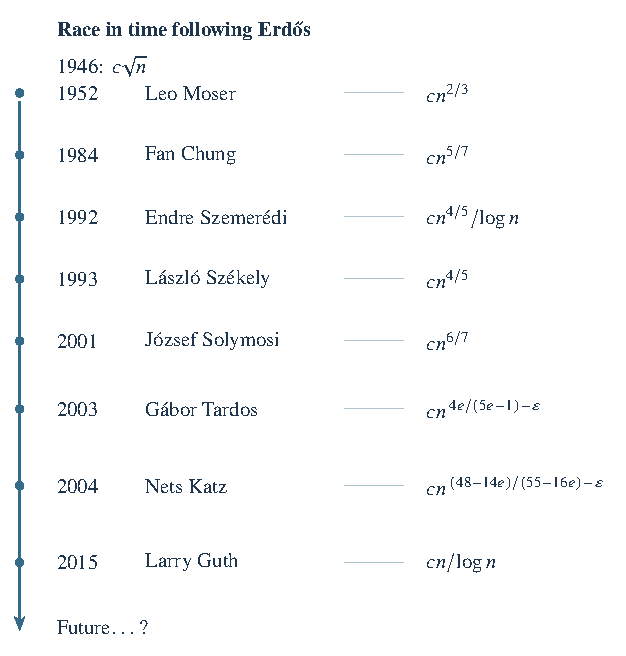
\includegraphics[width=.80\textwidth]{m2-fig-04.pdf}
 \FigureTag{M2.4}{fig:m2-fig-04}
\end{figure}
% Source page 12
Tools from Fourier analysis, number theory, graph theory, and even information
theory have gone into the formulation and resolution of this conjecture,
culminating in Guth's near-optimal result! We are just $1/\sqrt{\log n}$
away from Erd\H{o}s's conjecture. The future certainly shall bring hope.
% BLOG-CONTENT-END
\end{document}
